\documentclass[border=5pt]{standalone}
\usepackage{tikz}
\usetikzlibrary{arrows.meta, positioning, calc}

\begin{document}

\definecolor{accentblue}{RGB}{0, 120, 200}
\definecolor{accentred}{RGB}{220, 60, 20}
\definecolor{accentgrn}{RGB}{0, 150, 60}
\definecolor{labelgray}{RGB}{60, 60, 60}
\begin{tikzpicture}[
    lbl/.style={font=\small\bfseries, text=labelgray, align=center,
                fill=white, fill opacity=0.85, text opacity=1,
                rounded corners=2pt, inner sep=3pt},
    arr/.style={-{Stealth[length=2.5mm]}, line width=1pt, accentblue},
    stickbox/.style={font=\small\bfseries, align=center,
                     draw=accentblue, fill=accentblue!10,
                     rounded corners=3pt, inner sep=4pt},
  ]

  % Load controller photo
  % Path is relative to the main .tex that \input's this file
  \node[anchor=south west, inner sep=0] (img) at (0,0)
    {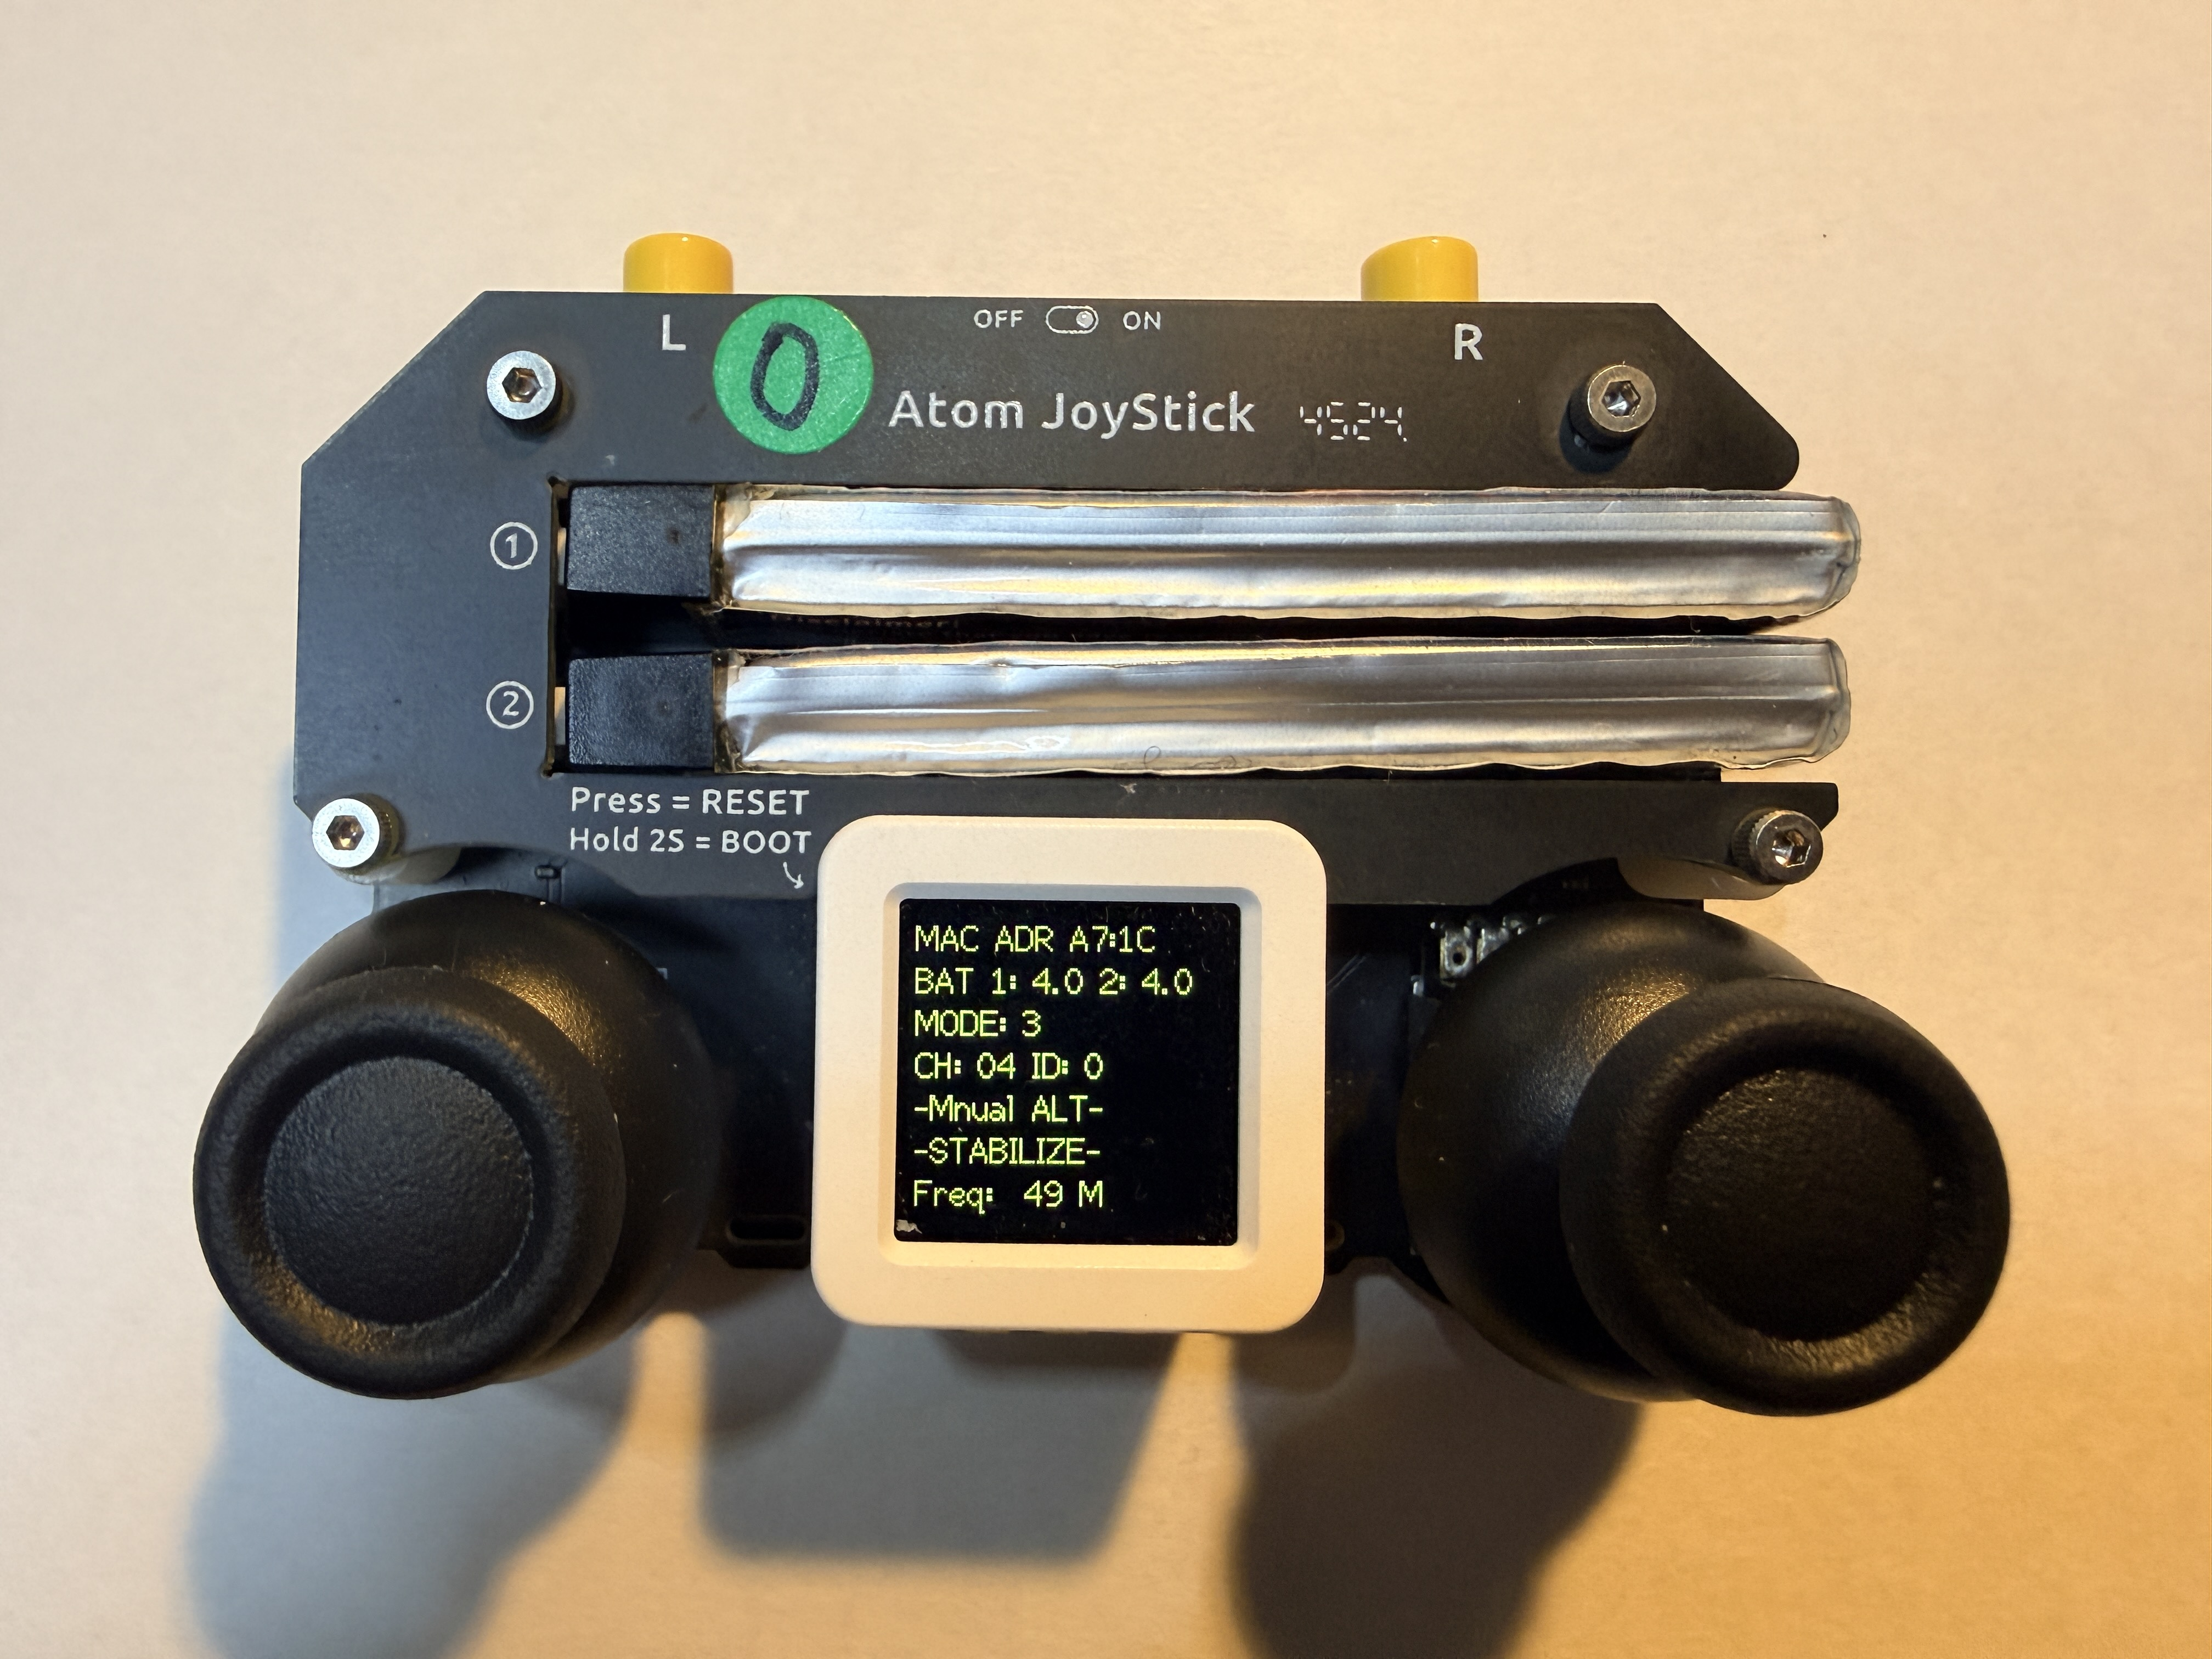
\includegraphics[width=10cm]{../images/controller.jpg}};

  % Set up relative coordinate system (0,0)-(1,1) over image
  \begin{scope}[
    x={(img.south east)},
    y={(img.north west)},
  ]

    % --- Left stick (MODE 3: Pitch / Roll) ---
    \node[stickbox, anchor=east] (lstick) at (-0.05, 0.28)
      {Pitch $\updownarrow$\\Roll $\leftrightarrow$};
    \draw[arr] (lstick.east) -- (0.18, 0.28);

    % --- Right stick (MODE 3: Throttle / Yaw) ---
    \node[stickbox, anchor=west] (rstick) at (1.05, 0.26)
      {Throttle $\updownarrow$\\Yaw $\leftrightarrow$};
    \draw[arr] (rstick.west) -- (0.82, 0.26);

    % --- Power switch ---
    \node[lbl, anchor=south] (pwr) at (0.53, 1.04) {Power SW};
    \draw[arr] (pwr.south) -- (0.53, 0.95);

    % --- M5 button (green) ---
    \node[lbl, anchor=south east] (m5) at (0.20, 1.04)
      {M5 Button\\{\footnotesize (Pairing)}};
    \draw[arr] (m5.south east) -- (0.35, 0.90);

    % --- Switch 1 ---
    \node[lbl, anchor=east] (sw1) at (-0.05, 0.68) {SW\,1};
    \draw[arr] (sw1.east) -- (0.10, 0.68);

    % --- Switch 2 ---
    \node[lbl, anchor=east] (sw2) at (-0.05, 0.56) {SW\,2};
    \draw[arr] (sw2.east) -- (0.10, 0.56);

    % --- LCD ---
    \node[lbl, anchor=north] (lcd) at (0.50, -0.06)
      {LCD\\{\footnotesize CH / MODE / BAT}};
    \draw[arr] (lcd.north) -- (0.50, 0.22);

    % --- MODE 3 badge ---
    \node[font=\footnotesize\bfseries, text=white,
          fill=accentred, rounded corners=2pt, inner sep=3pt,
          anchor=north east] at (1.05, 1.04) {MODE 3};

  \end{scope}
\end{tikzpicture}
\end{document}
